\documentclass[10pt,a4paper]{article}
\usepackage[utf8]{inputenc}
\usepackage[top=0.55in, bottom=0.55in, left=0.55in, right=0.55in]{geometry}
\usepackage{amsmath,amssymb}
\usepackage{listings}
\usepackage{xcolor}
\usepackage{hyperref}
\usepackage{enumitem}
\usepackage{booktabs}
\usepackage{tcolorbox}
\usepackage{tikz}
\usetikzlibrary{shapes,arrows.meta,positioning,calc,fit,backgrounds,matrix}

\definecolor{codegreen}{rgb}{0.12,0.55,0.22}
\definecolor{codegray}{rgb}{0.45,0.45,0.45}
\definecolor{codepurple}{rgb}{0.55,0,0.8}
\definecolor{backcolour}{rgb}{0.97,0.97,0.97}

\definecolor{boxblue}{RGB}{240, 246, 255}
\definecolor{borderblue}{RGB}{33, 114, 229}
\definecolor{boxorange}{RGB}{255, 248, 238}
\definecolor{borderorange}{RGB}{230, 126, 34}
\definecolor{boxgreen}{RGB}{240, 252, 242}
\definecolor{bordergreen}{RGB}{39, 174, 96}
\definecolor{boxpurple}{RGB}{250, 244, 255}
\definecolor{borderpurple}{RGB}{142, 68, 173}

% Tight spacing for printing
\setlist{nosep, leftmargin=1.1em}
\setlength{\parskip}{2.5pt}
\setlength{\parindent}{0pt}

\tcbset{
    colback=white,
    colframe=black!75,
    arc=2pt,
    left=5pt,
    right=5pt,
    top=3pt,
    bottom=3pt,
    boxrule=0.6pt,
    fonttitle=\bfseries\small
}

\lstdefinestyle{mystyle}{
    backgroundcolor=\color{backcolour},   
    commentstyle=\color{codegreen},
    keywordstyle=\color{blue}\bfseries,
    numberstyle=\tiny\color{codegray},
    stringstyle=\color{codepurple},
    basicstyle=\ttfamily\scriptsize,
    breakatwhitespace=false,         
    breaklines=true,                 
    captionpos=b,                    
    keepspaces=true,                 
    numbers=none,                    
    showspaces=false,                
    showstringspaces=false,
    showtabs=false,                  
    tabsize=2
}
\lstset{style=mystyle}

\tikzstyle{block} = [rectangle, draw=borderblue, fill=boxblue, rounded corners=2pt, text centered, minimum height=0.6cm, minimum width=1.9cm, font=\scriptsize\bfseries]
\tikzstyle{orangeblock} = [rectangle, draw=borderorange, fill=boxorange, rounded corners=2pt, text centered, minimum height=0.6cm, minimum width=1.9cm, font=\scriptsize\bfseries]
\tikzstyle{greenblock} = [rectangle, draw=bordergreen, fill=boxgreen, rounded corners=2pt, text centered, minimum height=0.6cm, minimum width=1.9cm, font=\scriptsize\bfseries]
\tikzstyle{purpleblock} = [rectangle, draw=borderpurple, fill=boxpurple, rounded corners=2pt, text centered, minimum height=0.6cm, minimum width=1.9cm, font=\scriptsize\bfseries]
\tikzstyle{circleop} = [circle, draw=black!80, fill=white, inner sep=1pt, font=\small\bfseries]
\tikzstyle{arrow} = [thick, ->, >=stealth]

\title{\vspace{-1.2cm}\textbf{\Large Building GPT from Scratch: Complete Architectural Reference, Code Explanation \& Viva Q\&A}\\\normalsize Companion to Andrej Karpathy's NanoGPT Lecture\vspace{-0.6cm}}
\author{\small Bakar -- NETSOL Internship Project}
\date{\vspace{-0.3cm}\small November 2026\vspace{-0.5cm}}

\begin{document}

\maketitle

\section{Introduction \& Repository Files}
A decoder-only autoregressive Transformer models the conditional probability $P(x_{t+1} \mid x_1, \dots, x_t)$ over a known vocabulary $\mathcal{V}$. At inference, it generates text by sampling next tokens autoregressively.
\begin{center}
\small
\begin{tabular}{@{}llp{11.5cm}@{}}
\toprule
\textbf{File} & \textbf{Stage} & \textbf{Description} \\ \midrule
\texttt{input.txt} & Dataset & 1,115,394 characters of Shakespeare plays ($|\mathcal{V}| = 65$). \\
\texttt{more.txt} & Validation Text & 10,000 characters of additional Shakespeare text for extended validation. \\
\texttt{bigram.py} & Baseline Milestone & Minimal model (~25:00 in video) predicting next token from current token alone. Zero history. \\
\texttt{train.ipynb} & Notebook & Interactive scratchpad with Versions 1--4 of self-attention, matrix operations, and training. \\
\texttt{v2.py} & Scaled Transformer & Full Transformer: 6 blocks, 6 heads, residuals, Pre-LN LayerNorm, dropout ($\sim$10.78M parameters). \\
\bottomrule
\end{tabular}
\end{center}

\vspace{-0.2cm}
\section{Decoder-Only GPT Architecture Flowchart}
\begin{center}
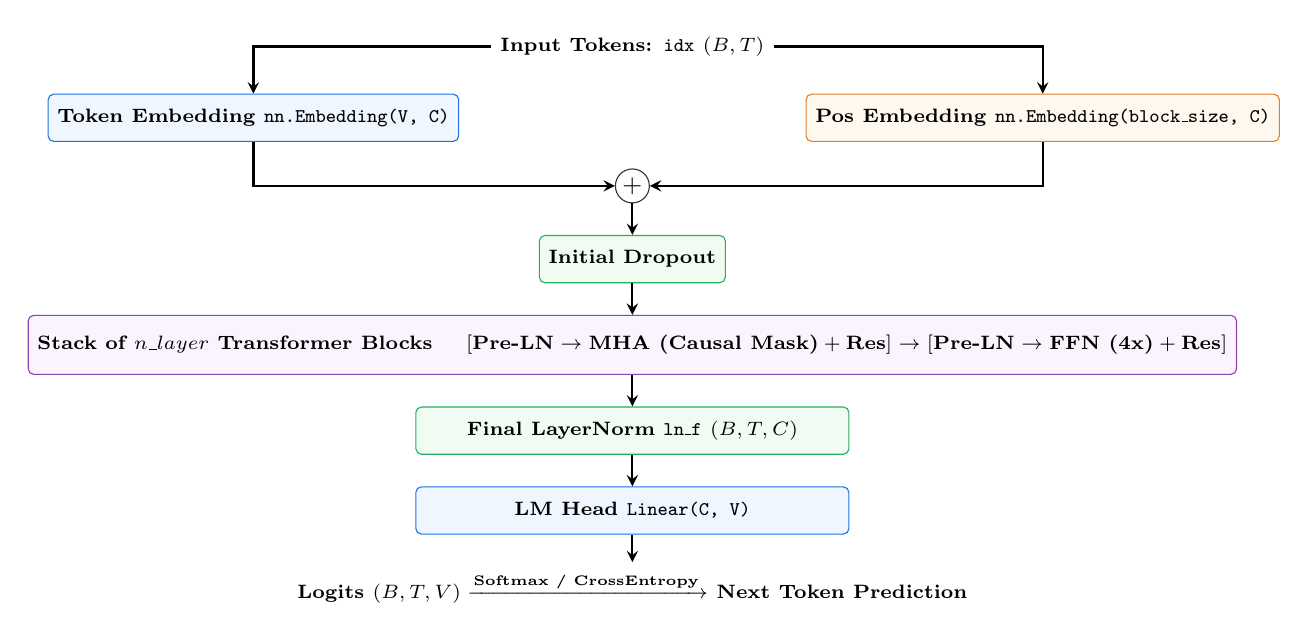
\begin{tikzpicture}[node distance=0.75cm, auto]
    \node (in) [font=\scriptsize\bfseries] {Input Tokens: \texttt{idx} $(B, T)$};
    \node (tok) [block, below left=0.35cm and 0.4cm of in] {Token Embedding \texttt{nn.Embedding(V, C)}};
    \node (pos) [orangeblock, below right=0.35cm and 0.4cm of in] {Pos Embedding \texttt{nn.Embedding(block\_size, C)}};
    \node (add1) [circleop, below=1.3cm of in] {$+$};
    \node (drop0) [greenblock, below=0.4cm of add1] {Initial Dropout};
    \node (block1) [purpleblock, below=0.4cm of drop0, minimum width=8.2cm, minimum height=0.75cm] {
        \textbf{Stack of $n\_layer$ Transformer Blocks} $\quad \left[\text{Pre-LN} \to \text{MHA (Causal Mask)} + \text{Res}\right] \to \left[\text{Pre-LN} \to \text{FFN (4x)} + \text{Res}\right]$
    };
    \node (lnf) [greenblock, below=0.4cm of block1, minimum width=5.5cm] {Final LayerNorm \texttt{ln\_f} $(B, T, C)$};
    \node (lmhead) [block, below=0.4cm of lnf, minimum width=5.5cm] {LM Head \texttt{Linear(C, V)}};
    \node (logits) [font=\scriptsize\bfseries, below=0.35cm of lmhead] {Logits $(B, T, V) \xrightarrow{\text{Softmax / CrossEntropy}}$ Next Token Prediction};

    \draw [arrow] (in) -| (tok);
    \draw [arrow] (in) -| (pos);
    \draw [arrow] (tok) |- (add1);
    \draw [arrow] (pos) |- (add1);
    \draw [arrow] (add1) -- (drop0);
    \draw [arrow] (drop0) -- (block1);
    \draw [arrow] (block1) -- (lnf);
    \draw [arrow] (lnf) -- (lmhead);
    \draw [arrow] (lmhead) -- (logits);
\end{tikzpicture}
\end{center}

\vspace{-0.3cm}
\section{Line-by-Line Code Explanation of Every Module}

\subsection{1. Data Preparation \& Tokenizer}
\begin{lstlisting}[language=Python]
chars = sorted(list(set(text))) # Extracts all 65 unique characters
vocab_size = len(chars)         # Size of vocabulary |V| = 65
stoi = {ch: i for i, ch in enumerate(chars)} # Dictionary mapping character to integer
itos = {i: ch for i, ch in enumerate(chars)} # Dictionary mapping integer to character
encode = lambda s: [stoi[c] for c in s]      # String -> list of integers
decode = lambda l: ''.join([itos[i] for i in l]) # List of integers -> String
data = torch.tensor(encode(text), dtype=torch.long) # Entire text stored as 1D long tensor
train_data = data[:int(0.9 * len(data))] # First 90% for training
val_data = data[int(0.9 * len(data)):]   # Remaining 10% for measuring generalization
\end{lstlisting}
\textbf{Explanation:} Karpathy builds a character-level tokenizer. $stoi$ assigns each character a token ID between 0 and 64. The full dataset is tokenized into a single 1D tensor and split 90/10 into train and validation sets.

\subsection{2. Batching \& Multi-Context Supervision (\texttt{get\_batch})}
\begin{lstlisting}[language=Python]
def get_batch(split):
    data = train_data if split == 'train' else val_data
    ix = torch.randint(len(data) - block_size, (batch_size,)) # Random starting offsets
    x = torch.stack([data[i:i+block_size] for i in ix])       # Inputs of shape (B, T)
    y = torch.stack([data[i+1:i+block_size+1] for i in ix])   # Targets shifted by 1 (B, T)
    return x.to(device), y.to(device)
\end{lstlisting}
\textbf{Explanation:} Random starting indices $ix$ grab chunks of length $T = block\_size$. Target $y$ is identical to $x$ but shifted forward by 1 character. For example, if $x = [\text{'h', 'e', 'l'}]$, then $y = [\text{'e', 'l', 'l'}]$. This simultaneously trains the model to predict next characters for all context lengths $1 \dots T$.

\subsection{3. Scaled Self-Attention Head (\texttt{Head})}
\begin{lstlisting}[language=Python]
class Head(nn.Module):
    def __init__(self, head_size):
        super().__init__()
        self.key = nn.Linear(n_embd, head_size, bias=False)   # What this token contains
        self.query = nn.Linear(n_embd, head_size, bias=False) # What this token is looking for
        self.value = nn.Linear(n_embd, head_size, bias=False) # Information this token communicates
        self.register_buffer('tril', torch.tril(torch.ones(block_size, block_size))) # Lower-triangular mask
        self.dropout = nn.Dropout(dropout)
    def forward(self, x):
        B, T, C = x.shape
        k = self.key(x)   # (B, T, head_size)
        q = self.query(x) # (B, T, head_size)
        # Compute affinities: (B, T, hs) @ (B, hs, T) -> (B, T, T) scaled by 1/sqrt(hs)
        wei = q @ k.transpose(-2, -1) * (k.shape[-1]**-0.5)
        # Causal mask: fill future positions with -inf so tokens cannot peek ahead
        wei = wei.masked_fill(self.tril[:T, :T] == 0, float('-inf'))
        wei = self.dropout(F.softmax(wei, dim=-1)) # Softmax normalizes weights to sum to 1
        return wei @ self.value(x) # Weighted aggregation: (B, T, T) @ (B, T, hs) -> (B, T, hs)
\end{lstlisting}
\textbf{Line-by-Line Explanation:}
\begin{itemize}
    \item \texttt{self.key, query, value}: Three linear layers projecting from embedding dimension $C$ to $head\_size$ without bias terms.
    \item \texttt{register\_buffer('tril', ...)}: A constant non-trainable tensor saved in the model state dictionary, holding the causal lower-triangular matrix.
    \item \texttt{q @ k.transpose(-2, -1)}: Performs batch matrix multiplication measuring affinity between every query token $i$ and key token $j$.
    \item \texttt{* (k.shape[-1]**-0.5)}: Multiplies by $1/\sqrt{d_k}$. This keeps dot-product variance at 1.0, preventing softmax from spiking into saturation.
    \item \texttt{masked\_fill(tril == 0, -inf)}: Future positions ($j > i$) become $-\infty$, ensuring $e^{-\infty} = 0$ in softmax so the model cannot look into the future.
    \item \texttt{wei @ self.value(x)}: Performs weighted average over value vectors $V$, returning the updated contextual representation.
\end{itemize}

\subsection{4. Multi-Head Attention (\texttt{MultiHeadAttention})}
\begin{lstlisting}[language=Python]
class MultiHeadAttention(nn.Module):
    def __init__(self, num_heads, head_size):
        super().__init__()
        self.heads = nn.ModuleList([Head(head_size) for _ in range(num_heads)]) # h parallel heads
        self.proj = nn.Linear(n_embd, n_embd) # Linear projection layer to mix head outputs
        self.dropout = nn.Dropout(dropout)
    def forward(self, x):
        out = torch.cat([h(x) for h in self.heads], dim=-1) # Concatenate over channel dimension (B, T, C)
        return self.dropout(self.proj(out))                 # Linear projection + dropout
\end{lstlisting}
\textbf{Explanation:} Applies $h$ attention heads in parallel ($d_k = C/h$). Each head specializes in a different linguistic relationship (e.g. grammar, rhyming, consonants). Their outputs are concatenated along the feature dimension and passed through a projection matrix $W_O$ to blend the learned features.

\subsection{5. Feed-Forward Network (\texttt{FeedForward})}
\begin{lstlisting}[language=Python]
class FeedForward(nn.Module):
    def __init__(self, n_embd):
        super().__init__()
        self.net = nn.Sequential(
            nn.Linear(n_embd, 4 * n_embd), # 4x expansion in hidden dimension
            nn.ReLU(),                     # Non-linear activation
            nn.Linear(4 * n_embd, n_embd), # Project back to embedding dimension
            nn.Dropout(dropout)
        )
    def forward(self, x): return self.net(x)
\end{lstlisting}
\textbf{Explanation:} Attention is the \textbf{communication} step where tokens share information. The Feed-Forward network is the \textbf{computation} step where each token reflects individually on what it gathered. Per the original Transformer paper, the inner linear layer expands the channel dimension $4\times$ ($C \to 4C$) before projecting back ($4C \to C$).

\subsection{6. Transformer Block (\texttt{Block}) with Pre-LN \& Residuals}
\begin{lstlisting}[language=Python]
class Block(nn.Module):
    def __init__(self, n_embd, n_head):
        super().__init__()
        self.sa = MultiHeadAttention(n_head, n_embd // n_head) # Communication layer
        self.ffwd = FeedForward(n_embd)                        # Computation layer
        self.ln1 = nn.LayerNorm(n_embd)                        # Pre-LayerNorm before attention
        self.ln2 = nn.LayerNorm(n_embd)                        # Pre-LayerNorm before FFN
    def forward(self, x):
        x = x + self.sa(self.ln1(x))   # Residual skip connection 1
        x = x + self.ffwd(self.ln2(x)) # Residual skip connection 2
        return x
\end{lstlisting}
\textbf{Line-by-Line Explanation:}
\begin{itemize}
    \item \texttt{x = x + self.sa(self.ln1(x))}: First, LayerNorm normalizes features across channels. Multi-Head Attention is applied, and the result is added back to original $x$ via the residual skip connection.
    \item \texttt{x = x + self.ffwd(self.ln2(x))}: Normalizes again, passes through Feed-Forward, and adds to $x$ via the second residual skip connection.
    \item \textbf{Why Pre-LN?} Modern GPT applies normalization \textit{before} transformations, keeping the residual identity highway ($x + \dots$) clean and un-normalized for stable gradient flow.
\end{itemize}

\subsection{7. Full Language Model Pipeline (\texttt{GPTLanguageModel})}
\begin{lstlisting}[language=Python]
class GPTLanguageModel(nn.Module):
    def __init__(self):
        super().__init__()
        self.token_embedding_table = nn.Embedding(vocab_size, n_embd)     # Content lookup
        self.position_embedding_table = nn.Embedding(block_size, n_embd) # Position lookup
        self.blocks = nn.Sequential(*[Block(n_embd, n_head=n_head) for _ in range(n_layer)]) # N blocks
        self.ln_f = nn.LayerNorm(n_embd)        # Final layer normalization
        self.lm_head = nn.Linear(n_embd, vocab_size) # Final projection to logits
    def forward(self, idx, targets=None):
        B, T = idx.shape
        tok_emb = self.token_embedding_table(idx) # (B, T, C)
        pos_emb = self.position_embedding_table(torch.arange(T, device=device)) # (T, C)
        x = tok_emb + pos_emb # Add content and positional coordinates (B, T, C)
        x = self.blocks(x)    # Pass through N Transformer blocks (B, T, C)
        x = self.ln_f(x)      # Final LayerNorm (B, T, C)
        logits = self.lm_head(x) # Project from C to vocab_size: (B, T, vocab_size)
        if targets is None:
            return logits, None
        B, T, C = logits.shape
        # Flatten (B, T) into 1D for cross entropy loss
        loss = F.cross_entropy(logits.view(B*T, C), targets.view(B*T))
        return logits, loss
    def generate(self, idx, max_new_tokens):
        for _ in range(max_new_tokens):
            idx_cond = idx[:, -block_size:] # Crop context window to block_size
            logits, loss = self(idx_cond)   # Forward pass
            logits = logits[:, -1, :]       # Focus only on the last token position: (B, vocab_size)
            probs = F.softmax(logits, dim=-1) # Convert logits to probabilities
            idx_next = torch.multinomial(probs, num_samples=1) # Sample next token (B, 1)
            idx = torch.cat((idx, idx_next), dim=1)            # Append to running sequence (B, T+1)
        return idx
\end{lstlisting}
\textbf{Line-by-Line Explanation:}
\begin{itemize}
    \item \texttt{tok\_emb + pos\_emb}: Tokens are given both semantic meaning and positional coordinates.
    \item \texttt{logits.view(B*T, C)}: \texttt{F.cross\_entropy} requires 2D input (samples $\times$ classes) and 1D target. We flatten batch and sequence length dimensions together.
    \item \texttt{idx[:, -block\_size:]}: If the generated text exceeds 256 tokens, positional embeddings would throw an IndexError. Cropping ensures the context window never exceeds \texttt{block\_size}.
    \item \texttt{torch.multinomial}: Samples from the probability distribution rather than always picking the highest probability (greedy search), allowing diverse and creative generation.
\end{itemize}

\vspace{-0.2cm}
\section{15 Professor / Viva Oral Examination Questions \& Answers}

\begin{tcolorbox}[title=Q1: What are logits, and why do we not apply softmax during training?]
\textbf{Answer:} Logits are raw, unnormalized prediction scores from the final linear layer. We pass raw logits directly to PyTorch's \texttt{F.cross\_entropy} because it mathematically fuses $\text{log-softmax}$ and negative log-likelihood into a single numerically stable kernel, preventing floating-point overflow and underflow.
\end{tcolorbox}

\begin{tcolorbox}[title=Q2: Why is the baseline initial loss approximately 4.17?]
\textbf{Answer:} Vocabulary $|\mathcal{V}| = 65$. At random initialization, predictions are uniform ($P = 1/65$). Cross-entropy loss is negative log-likelihood: $\mathcal{L}_{\text{init}} = -\ln(1/65) = \ln(65) \approx 4.174$. A starting loss near 4.17 proves tensor initialization is mathematically sound.
\end{tcolorbox}

\begin{tcolorbox}[title=Q3: Explain Query, Key, and Value conceptually and mathematically.]
\textbf{Answer:} Soft database lookup: \textbf{Query ($Q$)} is what a token seeks; \textbf{Key ($K$)} is what a token offers; \textbf{Value ($V$)} is the information passed along if they match. Dot product $Q K^T$ computes alignment scores, which weight how much of $V$ is pooled into the token representation.
\end{tcolorbox}

\begin{tcolorbox}[title=Q4: Why divide by $\sqrt{d_k}$ in scaled dot-product attention?]
\textbf{Answer:} For independent unit-variance vectors $q, k$, the dot product $\sum_{i=1}^{d_k} q_i k_i$ has variance $d_k$. For large $d_k$, scores explode in magnitude, pushing softmax into extreme saturated regions with near-zero gradients. Dividing by $\sqrt{d_k}$ preserves unit variance and healthy gradient flow.
\end{tcolorbox}

\begin{tcolorbox}[title=Q5: What is causal masking and why is it mandatory in GPT?]
\textbf{Answer:} In autoregressive modeling, predicting token $t+1$ must depend strictly on tokens $1 \dots t$. If future positions were accessible, the model would cheat by simply copying future characters rather than learning language. Causal masking sets future affinities ($j > i$) to $-\infty$, forcing softmax to assign them strictly 0 weight.
\end{tcolorbox}

\begin{tcolorbox}[title=Q6: Difference between Encoder Attention and Decoder Attention?]
\textbf{Answer:} Encoder attention (BERT) is bidirectional: every token attends to all past and future tokens (no causal mask). Decoder attention (GPT) is autoregressive: causal lower-triangular masking strictly blocks attention to future positions.
\end{tcolorbox}

\begin{tcolorbox}[title=Q7: Why do Transformers strictly require Positional Embeddings?]
\textbf{Answer:} Self-attention is permutation-equivariant: it computes pairwise affinities regardless of token sequence order. Scrambling words in a sentence yields identical attention representations. Positional embeddings inject sequence order by adding a unique coordinate vector to each position.
\end{tcolorbox}

\begin{tcolorbox}[title=Q8: Why use Multi-Head Attention instead of one large Single Attention Head?]
\textbf{Answer:} A single head collapses token affinities into one averaged pattern. Multi-Head Attention projects into $h$ distinct representation subspaces ($d_k = C/h$), allowing the model to simultaneously track grammar, rhyming, and semantics across heads at identical computational cost.
\end{tcolorbox}

\begin{tcolorbox}[title=Q9: What is the exact function of the Feed-Forward Network?]
\textbf{Answer:} Attention is \textbf{communication} (tokens exchanging context). The Feed-Forward network is \textbf{computation} (each token individually processing what it gathered). It applies a non-linear 2-layer MLP with 4x expansion ($C \to 4C \to C$), adding representational capacity.
\end{tcolorbox}

\begin{tcolorbox}[title=Q10: Why are Residual Connections critical for training deep Transformers?]
\textbf{Answer:} Gradients diminish exponentially when backpropagating through deep non-linear layers (vanishing gradients). Residual connections create identity bypass highways: $x_{l+1} = x_l + \mathcal{F}(x_l) \implies \frac{\partial x_{l+1}}{\partial x_l} = 1 + \mathcal{F}'(x_l)$. The $+1$ term lets gradients flow directly back without dying.
\end{tcolorbox}

\begin{tcolorbox}[title=Q11: Contrast Layer Normalization with Batch Normalization.]
\textbf{Answer:} Batch Normalization normalizes across the batch dimension ($B$) for each channel, coupling batch samples and failing on small batches. Layer Normalization normalizes across the channel dimension ($C$) for each token independently, making it batch-size invariant and ideal for sequence modeling.
\end{tcolorbox}

\begin{tcolorbox}[title=Q12: Why did modern GPT switch from Post-LN to Pre-LN?]
\textbf{Answer:} Original Transformer applied LayerNorm after residual addition (Post-LN: $x \leftarrow \text{LN}(x + \mathcal{F}(x))$). Gradients through un-normalized residual branches cause training instability. Modern GPT uses Pre-LN ($x \leftarrow x + \mathcal{F}(\text{LN}(x))$), preserving clean un-normalized identity skip paths.
\end{tcolorbox}

\begin{tcolorbox}[title=Q13: What does Dropout do, and where is it placed in GPT?]
\textbf{Answer:} Dropout randomly zeroes out activations with probability $p$ during training, preventing neurons from co-adapting and overfitting. Placed: 1) on attention weights matrix ($wei$), 2) after multi-head projection, and 3) after the Feed-Forward network.
\end{tcolorbox}

\begin{tcolorbox}[title=Q14: Detail the autoregressive text generation procedure at inference time.]
\textbf{Answer:} 1) Crop context to last $block\_size$ tokens; 2) Forward pass to get logits $(B, T, V)$; 3) Extract final time step logits $(B, V)$; 4) Apply softmax to get probabilities; 5) Sample next token index via \texttt{torch.multinomial(probs, 1)}; 6) Concatenate sampled token to running sequence and repeat.
\end{tcolorbox}

\begin{tcolorbox}[title=Q15: What distinguishes our model from production GPT-2 / GPT-3?]
\textbf{Answer:} 1) \textbf{Tokenization:} Character-level (65 tokens) vs. Byte-Pair Encoding (BPE, $\sim 50\text{k}$ tokens); 2) \textbf{Scale:} 10.7M parameters vs. 124M (GPT-2 small) and 175B (GPT-3); 3) \textbf{Data:} 1MB Shakespeare vs. hundreds of gigabytes of web crawl data.
\end{tcolorbox}

\vspace{-0.2cm}
\section{Hyperparameter Matrix \& Real Colab Results}
\begin{center}
\small
\begin{tabular}{@{}lccc@{}}
\toprule
\textbf{Parameter} & \textbf{Bigram Baseline} & \textbf{Notebook Scratchpad} & \textbf{Final Model (\texttt{v2.py})} \\ \midrule
Batch Size ($B$) & 32 & 16 & 64 \\
Block Size ($T$) & 8 & 32 & 256 \\
Embedding Dimension ($C$) & -- & 64 & 384 \\
Heads ($h$) / Head Dim ($d_k$) & -- & 4 / 16 & 6 / 64 \\
Layers ($n\_layer$) & 0 & 4 & 6 \\
Parameters & 4,225 & 209,729 ($\sim$210K) & 10,788,929 ($\sim$10.78M) \\
Validation Loss & $\sim 2.50$ & $\sim 2.45$ & \textbf{1.5541} (Train: \textbf{0.8583}) \\
Hardware Tested & CPU & CPU & Colab GPU (T4 / A100) \\ \bottomrule
\end{tabular}
\end{center}

\textbf{Sample Shakespeare Generated by Our Model in Colab Run:}
\begin{quote}
\scriptsize\ttfamily
CORIOLANUS: That I would do but out the other side hourly I'll proceed to him dearly. I was't come forth, to make yourselves as the penenyworth. | VOLUMNIA: By my remedied with my name? | CORIOLANUS: For I am cratch with thyself, but as I will reconfuse hurr. | MARCIUS: To end the night him too reason to the people. Here's this, and cause the kittest for this friend.
\end{quote}

\end{document}
